\section{Groups in the World}

\vspace{4mm}

\subsection*{The Church of the Seven}

The Church is the dominant political, military, and spiritual power in Velterra.  Founded to serve the will of the Seven Gods, the Church has ruled the known world for centuries through a network of pastors, arbiters, and inquisitors.  Since the Sundering --- when the Church used the Great Stone to sever the world's connection to the divine --- the institution has grown increasingly corrupt, wielding the filtered remnants of godly power to maintain control.

The Church's hierarchy stretches from humble village pastors to the fearsome Arbiters who enforce divine law, and at its darkest reaches, the shadowy Inquisition --- an elite force of divine warriors who hunt down heretics and enemies of the faith with terrifying efficiency.

The Church views magic with deep suspicion and actively suppresses knowledge that contradicts its teachings, leading to the creation and eventual purge of the Book Burners.

\subsection*{The Jennies}

\begin{center}
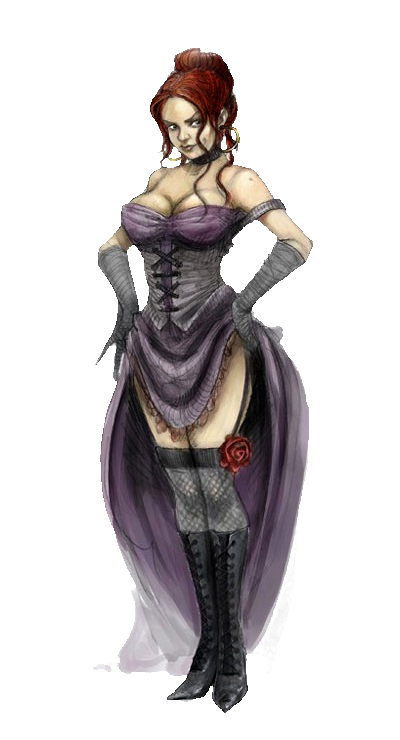
\includegraphics[width=80mm]{./content/img/jennies3.png}
\begin{figure}[h]
\end{figure}
\end{center}

The Jennies are a group of ladies who offer discrete services for the discerning adventurer.  Originally a network of courtesans, the Jennies were forced underground when the Church officially outlawed their profession.  Under the leadership of Mae Harkwood, they reinvented themselves as a formidable criminal organisation, spreading ``like herpes through the empire''.

Operating from a hidden camp known affectionately as ``Whorecity'', the Jennies proved to be surprisingly capable allies.  Delilah, one of their finest operatives, joined the party early in their adventure and went on to become Riphard's wife, the Sky Captain of Tomorrow, and one of the group's most reliable fighters.  Mae herself helped the group track down both the SRA and Diego Escabar's bandits.

\smallskip

\subsection*{The SRA --- Small Rights Activists}

\begin{center}
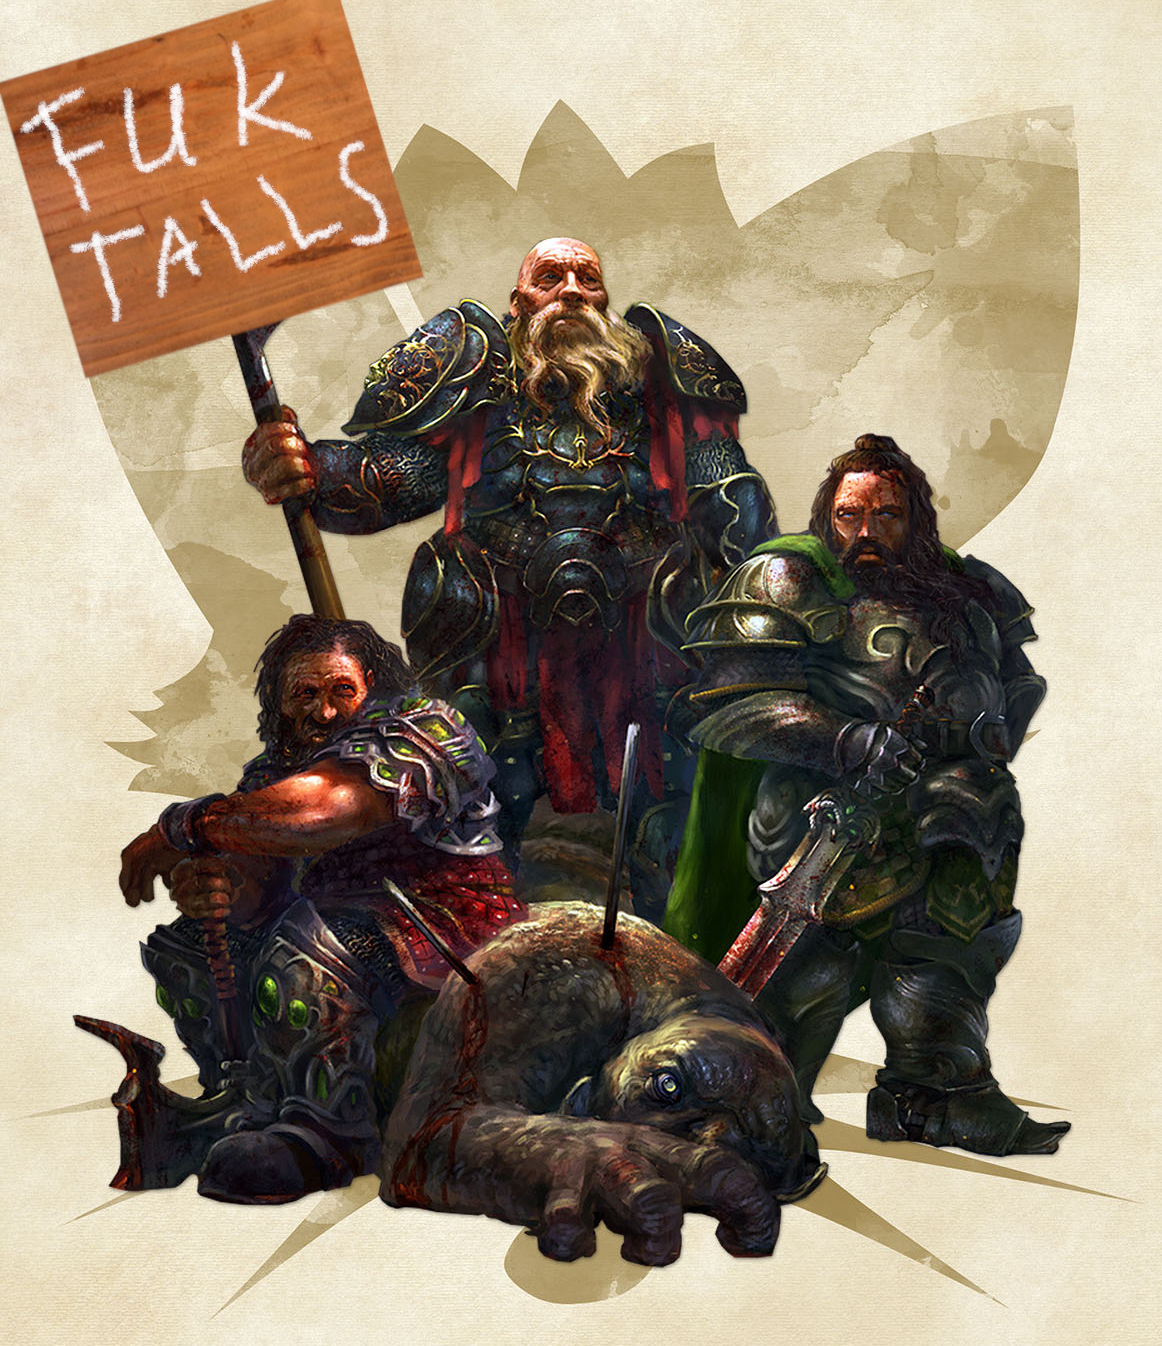
\includegraphics[width=80mm]{./content/img/sra3.jpg}
\begin{figure}[h]
\end{figure}
\end{center}

A collection of mainly gnomes and halflings who perform terrorist acts in their quest for improving the rights of smaller folk.  Led by Razzle Backshine --- a gnome with a penchant for exploding things in people's faces --- the SRA was spread across the empire conducting increasingly volatile operations.

The party's encounter with the SRA was characteristically complicated.  After infiltrating Razzle's hideout through a combination of forged documents, elaborate deception, and Exme's railgun, the group killed Razzle and installed ``Buttons'' as the new leader of the faction, hoping to redirect the organisation toward less indiscriminate violence.

\smallskip

\subsection*{The Book Burners}

\begin{center}

\includegraphics[width=80mm]{./content/img/bookBurner.jpg}
\begin{figure}[h]
\end{figure}
\end{center}

The Book Burners were the Church's sanctioned order of literary enforcers, tasked with hunting down and destroying heretical texts.  Part mercenary company, part secret police, the Book Burners operated under Church authority to suppress dangerous knowledge.

The organisation's downfall came from within.  Members like Pilcheur Gamont were secretly selling books instead of burning them, and when the Church discovered this betrayal, they launched a brutal purge that scattered the surviving Book Burners across the continent.  Their former headquarters in Hope's Rest was eventually claimed by the party and repurposed as the Gary Guild's base of operations, complete with firepoles and a vault.

Key former members include Pilcheur, Burnie Cinders, Lillian (a half-elf who fled west), Zippy (an alcoholic gnome), and Archibald --- the elderly, near-blind librarian who continued to tend the abandoned headquarters long after everyone else had fled.

\smallskip

\subsection*{The Gary Guild}

The Gary Guild --- officially ``Garys Against Religion, Yo'' --- was founded by the party in Hope's Rest as a front for their anti-Church operations.  What began as an absurd proposition by a stone man in a flowery outfit became a genuine political force in the city.

The guild secured its headquarters through a dramatic guild council vote, with Gary's impassioned speech winning over the assembled guild masters.  They formed a joint venture with the Guilds of Services, Might, and Life, and established themselves as a legitimate presence in the city's power structure.

The guild's logo, drawn by Gary himself, was described as ``a universal hit''.  Derek Bobacious was recruited to manage the guild's marketing operations, employing billboard campaigns with slogans like ``We Take Interest in Your Interest''.

\smallskip

\subsection*{The Bank}

Founded by Riphard Obsidian Hardstone, the Guild of Banking was Velterra's first financial institution.  It began humbly in the house of Derek Bobacious in Riverfall --- an elderly bachelor who was convinced that ``the gods want to run a shop in his house'' --- and grew into a full guild operation in Hope's Rest.

The bank's pitch --- ``Safe Storage for a Dangerous World'' --- impressed the Guild of Coin's head, Rowlett Marnett, enough to secure investment.  Key positions included Riphard as Head Interface Officer, Gary as Global Business Unification Investigator, Delilah as Job Organiser (Lower Klass), Pilch as Quota, Rosta, Training and Torture Officer, Exme as Untrustworthy Individual, and Kolo as Grossly Untrustworthy Individual.

\smallskip

\subsection*{The Hearthrust Society}

Founded by Lady Otoria Hearthrust before her death, the Hearthrust Society is an emancipation movement of robot ladies from Nanduan.  Built by a craftsman named Konrad, these automata --- including Lady Vashen, Lady Hirota, and Lady Averio --- fight for freedom and autonomy.

Otoria had killed the Emperor of Masuda and founded the Society before fleeing to Velterra, leaving behind a network of mechanical women who would carry on her cause.  The Society allied with the party during the Masuda campaign, providing a robot army that proved decisive in several key battles.  Lady Hirota personally rescued the group from certain death by swooping in on a mechanical eagle.

For the final assault on Seven's Spire, the Hearthrust Society sent their female ninja riders on mechanical eagles to join the alliance army --- a fitting tribute to the woman whose principles of honour and emancipation had inspired them all.

\smallskip

\subsection*{The Inquisition}

The Church's elite secret enforcement arm.  Dark masked figures with tentacle maws instead of mouths, the Inquisitors are the most terrifying force in Velterra.  Each bears a Canilon tattoo under their chest --- a symbol connected to the elder entity Kalimar.

Inquisitors are immune to all non-Excalibrum weapons, making them effectively invincible against conventional forces.  Their existence is officially denied by the Church, which makes their habit of publicly executing people somewhat awkward.  The party's first encounters with the Inquisition were one-sided affairs that ended in retreat; only after forging Excalibrum weapons could they fight on equal terms.

The most dangerous variant --- the Inquisitor Ravagers --- are massive hulking beings with rough-hewn metal spikes inserted where hands should be.  Two of these accompanied Arbiter Khan in the final encounter at Seven's Spire.

\smallskip

\subsection*{The Varg}

A northern warlord and barbarian alliance that dominates the frozen lands beyond Linderdorf.  The Varg enslaved the goblin tribes, including Kolo and Exme's people, and maintain control through roving bands of bearkin warriors.  Their territory is a bitter, snowbound wasteland where children watch travellers from the hills and the Varg Hold stretches for miles as a massive tent city.

The historical figure Hunthar Varg once led an incursion into Church territory that was only stopped by the Zealot Arbiter Elron wielding the Hammer of the Gods.  In the present day, the Varg remain a threat to civilised lands, with Linderdorf serving as the bastion against their raids.

\smallskip

\subsection*{The University of Assassins}

Part educational institution, part criminal enterprise.  The University operates in Hope's Rest under the Guild of Services, training students in the arts of stealth, poison, and targeted elimination.  Burnie once held a teaching position there, and his son Buck McCraw now trains students --- including Kevin, the final-year PhD student who joined the party to complete his fieldwork requirements.

The University's clockwork ninja assassins joined the alliance army for the final battle at Hope's Rest, proving that even contract killers can be moved by a good cause --- or at least a sufficiently large payment.

\smallskip

\subsection*{The Alliance Army}

The coalition assembled for the final assault on the Church's power, built through every friendship, favour, and alliance the party had forged across years of adventuring.  The army comprised:

The Gary Guild and Hope's Rest commoners.  The Jennies.  Clockwork ninja assassins from the University.  Tom'ardy dwarves.  Linderdorf robots and cannons.  The Hearthrust Society's mechanical eagle riders.  New Abbergast's fishmen under King Oceani.  The Stonecast Mech, dropped from the airship as a siege weapon.

Their assault on Seven's Spire was the culmination of the party's mission --- friendship really was magic, after all.

\smallskip

\subsection*{Hell Inc.}

Hell is not merely a place of torment --- it is a bureaucracy.  Managed by the devil Lazarus from his plush office (accessible via portal doors created by Meredith, his elephantine butler), Hell operates with departmental efficiency: demons handle the torturing, devils handle the bookkeeping.

Lazarus recruited the party because the Church's ever-expanding definition of sin was flooding Hell with undeserving souls, overwhelming the system.  His war room --- complete with a large-scale map of Velterra and intelligence on Church troop movements --- became the party's strategic command centre in the final campaign.  His superior, Arbigal, used ``brutal underhanded management tactics'' to gain control of the operation.

Following the return of the Gods, Lazarus was rewarded for his efforts by being re-ascended into his full angel form.

\smallskip

\bigskip

\clearpage
